\section{Analysis}
\label{sec:analysis}

Beyond overall performance, we further analyze why \method{} is
effective as a semantic search framework for alpha mining. Our analyses
focus on four aspects: (1) whether the proposed schema decomposition
provides meaningful semantic structure for factor discovery; (2) whether
the trading-semantic space contains learnable reward information and can
be effectively navigated during search; (3) how realization budget should
be allocated under stochastic plan-to-factor mapping; and (4) whether the
framework remains robust across different LLM realization backends.
\subsection{Semantic Component Ablation}

We first examine whether individual schema components provide useful
information for factor discovery. Unless otherwise noted, all variants
share the same LLM backend and evaluation protocol.

\begin{figure}[!t] \centering 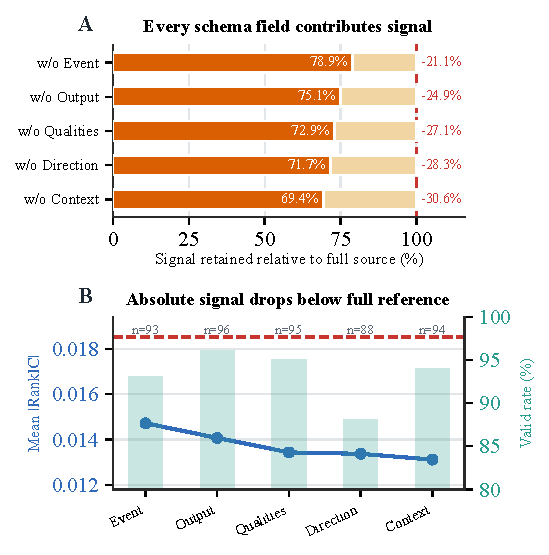
\includegraphics[width=\columnwidth]{figures/schema_component_ablation.pdf} \caption{Component-wise schema ablation.} \label{fig:schema_leave_one_out} \end{figure}

We select 100 complete schema plans and construct five
leave-one-component-out variants by removing one field from
\(\{\emph{Event}, \emph{Context}, \emph{Qualities}, \emph{Direction},
\emph{Output}\}\). Each incomplete plan is provided to DeepSeek-V4-Flash
for factor realization, with one repair opportunity allowed under the
same execution protocol. The generated factors are then evaluated after
execution validation and backtesting.

Figure~\ref{fig:schema_leave_one_out} summarizes the results. Removing
any schema component leads to a degradation in factor quality, while
the implementation success rate decreases only moderately. Here,
successful implementation requires passing execution checks including
data-contract compliance, numerical validity, and look-ahead leakage
screening. The relatively small drop in validity suggests that the LLM
can still construct executable factors even from incomplete semantic
descriptions, but the missing components reduce the quality of the
resulting factors.

Across all leave-one-out variants, removing a single semantic component
causes a clear reduction in Rank IC compared with the complete schema
plans. This indicates that the five schema dimensions provide
complementary information for factor discovery: although the realization
model can compensate for missing semantic details, the resulting factors
are less effective when important aspects of the trading mechanism are
omitted.


\subsection{Backend Robustness Analysis}

We test whether schema-guided realization depends on a single implementation agent. Holding 100 schema plans fixed, six code-agent backends implement the same plans, with at most one retry for failed cases when available. Final success rates range from 82\% to 99\%, while mean \(|\mathrm{RankIC}|\) over successful implementations remains in a comparable range (0.0116--0.0168). Figure~\ref{fig:code_agent_model_invariance} separates these two effects: Panel A reports pass@1 success and repair recovery, and Panel B reports post-success signal quality. The result suggests that backend choice mainly affects execution reliability, while the semantic plan and the resulting factor function transfer across different code agents. Appendix~\ref{sec:appendix_code_agent_robustness} provides the full table.

\begin{figure}[!t]
    \centering
    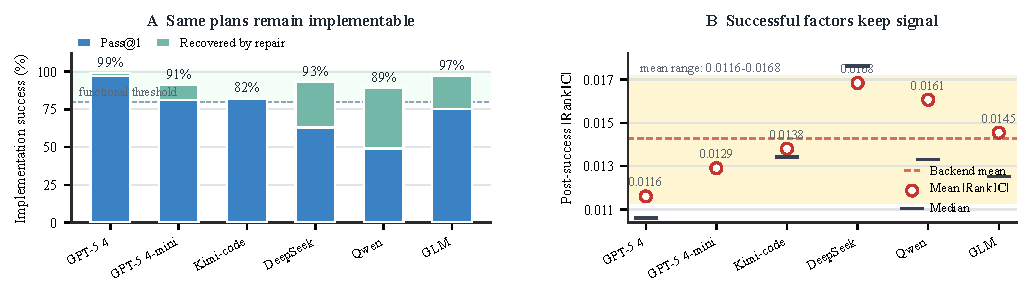
\includegraphics[width=\columnwidth]{figures/code_agent_model_invariance.pdf}
    \caption{Repair-aware robustness to code-agent backends on the same 100 schema plans. Panel A separates first-attempt implementation success from repair recovery; Panel B shows that successful implementations retain comparable signal quality across backends.}
    \label{fig:code_agent_model_invariance}
\end{figure}

\subsection{Schema-Space Predictability Analysis}

We further ask whether schema rewards are predictable before code realization. We collect 12,126 historical plan--reward pairs covering 11,295 unique schema keys and train lightweight predictors using only discrete schema features. \emph{Single schema} uses component-level indicators and category/scope counts, while \emph{Schema + pair} additionally includes pairwise component interactions. No schema text embeddings, generated code, factor values, or backtest trajectories are used as inputs.

\begin{figure}[!t]
    \centering
    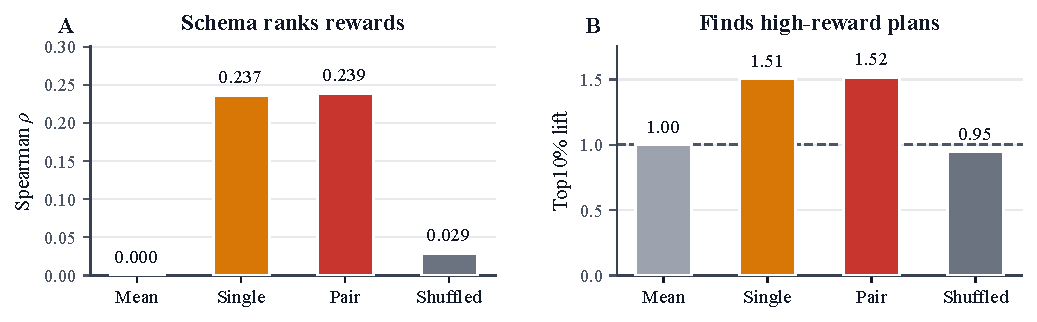
\includegraphics[width=\columnwidth]{figures/schema_space_predictability.pdf}
    \caption{Schema-space reward predictability.}
    \label{fig:schema_predictability}
\end{figure}

Figure~\ref{fig:schema_predictability} shows that schema-level features are predictive under this restricted setting. Panel A compares reward-ranking quality, while Panel B reports top-decile enrichment for the mean baseline, the single-schema LightGBM scorer, the pair-interaction LightGBM scorer, and the shuffled-reward control. Single-schema LightGBM reaches Spearman \(0.237\) and top-decile lift \(1.506\), while adding pair interactions improves the lift to \(1.519\). The mean baseline has no ranking ability, and the shuffled-reward control remains near random, indicating that the signal is tied to the true schema--reward association rather than model capacity alone.
